% !TEX root = OptimalOffline.tex

Concluding the results of all Lemmas our optimal policy $\{\textbf{p},\textbf{s},N\}$ must have change transmission powers at energy arrival epochs only i.e. $\forall i,\ s_i=t_j$ for some $j$. At these epochs we exhaust the total energy available with us i.e. $U(s_i^-)=\ETx(s_i^-)$. The transmission powers are also non decreasing with time and we exhaust the total 'receiver time' time given to us, if we do not start transmitting from origin.

Now that we have gained some knowledge of the structure our algorithm has to follow, we consider an example to approach Problem 1. 

Suppose we are given that the receiver can be \textit{on} for a maximum duration of $T$. Our goal is to find a transmission policy so that we can minimize the time at which the transmission is completed. To do this, we shall first find a feasible solution i.e. one which satisfies all constraints (\ref{pb1_constraint_bits})-(\ref{pb1_constraint_time}) and keep improving upon it, until we have a solution that follows all our Lemma 1-4 and hits the boundary on some or all of the constraints (\ref{pb1_constraint_bits})-(\ref{pb1_constraint_time}). 

We need an initial feasible solution to begin with. For this, we find the minimum energy required by the transmitter so that the transmission can be completed in duration $T$ with a constant power. That is, the first $\ETx(t_n)$ such that
\begin{equation}
T g\left(\frac{\ETx(t_n)}{T}\right)\geq B_0.
\end{equation}
Let $\widetilde{T}$ be the time duration such that
\begin{equation}
\widetilde{T}g\left(\frac{\ETx(t_n)}{\widetilde{T}}\right)=B_0.
\end{equation}
Let $p_c=\frac{\ETx(t_n)}{\widetilde{T}}$. We try to transmit with this power starting at time $t=0$. If it does not violate the energy constraint (\ref{pb1_constraint_energy}), we are done with the optimal solution and our transmission is completed in $\widetilde{T}$ time.

If not, we start the transmission as early as possible, such that the transmission is feasible with respect to (\ref{pb1_constraint_energy}). This transmission policy, will encounter atleast one epoch where total energy consumed till that epoch is equal to the total energy harvested upto it. Let time $t_q$ be the first point where this happens. This is shown in Fig. \ref{straight} .  Till now we have not argued why we chose such a policy to start with. In fact the Lemma \ref{lemma_Q} shows that this starting solution is a 'good' estimate of policy at and before time $t_q$, as both the optimal policy and the above policy run out of all their energy at epoch $t_q$. 

Now, according to Lemma \ref{lemma_energy_consumed}, the optimal policy must finish all available energy when it stops transmission. If transmitting with $p_c$ power does use up all the energy (Fig. \ref{straight} (b)), then we accept the constant power transmission with $p_c$ as our initial policy (line number \ref{init_policy_CP} in Algorithm \ref{init_policy}). If it does not finish up all of $\ETx(n)$ with $p_c$ power till the end (shown in Fig. \ref{straight} (b)), we should choose a better policy after time $t_q$. $p_c$ sends $\widetilde{B}$ amount of bits after $t_q$, which is calculated in line number \ref{init_policy_bits_t_q} of INIT\_POLICY. Now, we require our transmission policy to send $\widetilde{B}$ bits after time $t_q$, in as little time as possible (and of course, before $S$), keeping in mind that the policy should use all $\ETx(t_n)$ amount of energy till the end. Algorithm 1 in \cite{Yang} does the job for us. Hence in this case, we choose transmission with $p_c$ till $t_q$ and then the solution of Algorithm 1 in \cite{Yang} after time $t_q$. 

\begin{figure}
\label{straight}
\centering
  \centerline{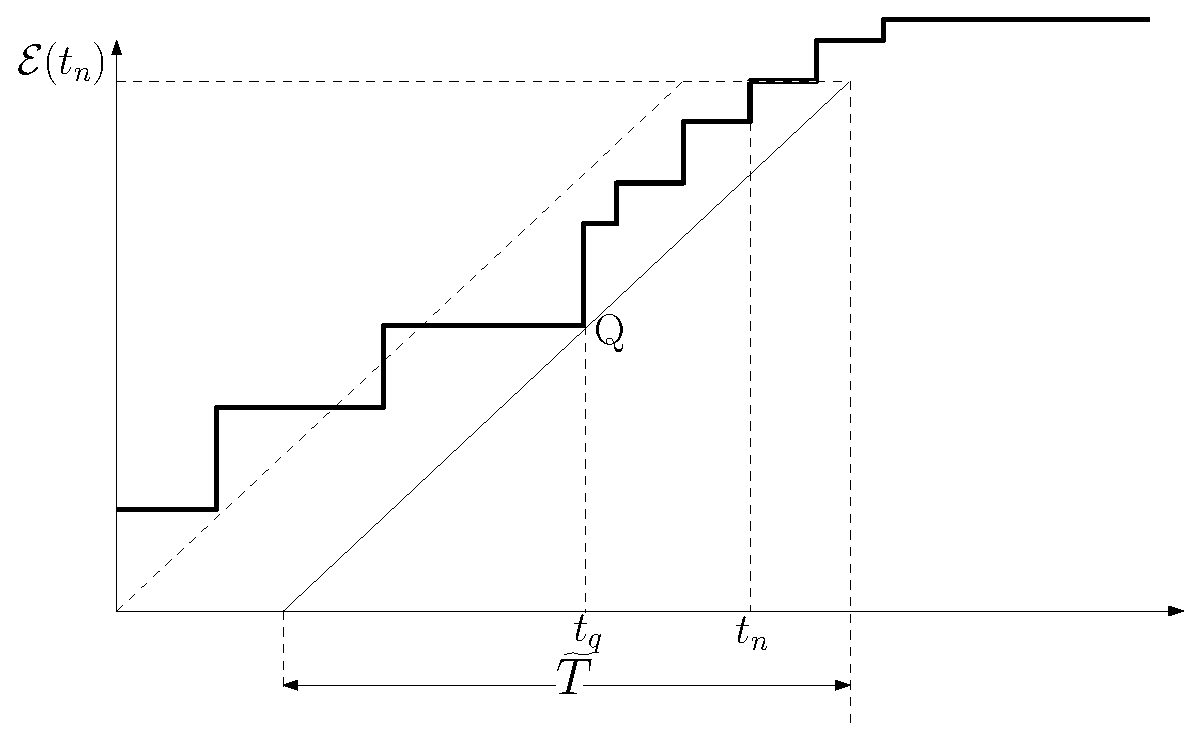
\includegraphics[width=8cm]{straight.eps}}
\caption{Figure showing point $t_q$.}
\end{figure}

\begin{lemma}
In every optimal solution, at energy arrival epoch $t_q$, $U(t_q^-)=\ETx(t_q^-)$.
\label{lemma_Q}
\end{lemma}
\begin{proof}
We shall prove this by contradiction. Let the start and end times of the constant power transmission policy described above be $R$ and $S$ receptively. We make the following claims:

\textbf{Claim 1:} Every optimal transmission policy begins transmission at or before time $R$

Since, $S-T=\widetilde{T}\le T$ (by Lemma \ref{transmission_duration}) if a transmission policy has to finish before $S$, it has to start before time $\max(S-T,0) \le \max(R,0)$. 

%Since we are transmitting all the bits at the maximum possible power, no policy that starts after $R$ can finish before $S$. Therefore, any policy that starts after $R$ cannot be optimal.

\textbf{Claim 2:} Every optimal transmission policy ends transmission at or before time $S$.
This follows immediately from the fact that the policy is optimal.

Let $t_q$ equal to time $t_i$ for some $i\in\mathbb{N}$. Suppose we have an optimal transmission policy that does not exhaust all its energy at time $t_q$ i.e. $U(t_j)<\ETx(t_i^-)$. By Lemma \ref{lemma_energy_consumed} it does not change its transmission power at $t_i$. Let the transmission power of optimal policy be $p$ at $t_i$. This does not change till an epoch, say $t_j$. Now, $t_j<S$ by \textit{Claim 2}. Further the constant power policy exhausts all its energy by $t_q$. So,
\begin{align}
&\tilde{p}(t_i-R)=\ETx(t_i^-)\label{eqlemmaQ1}.
\end{align}
But, by constraint (\ref{pb1_constraint_energy})
\begin{align}
&\tilde{p}(t_i-R)+\tilde{p}(t_j-t_i)\le \ETx(t_j^-),
\\
&\implies \tilde{p}(t_j-t_i)\stackrel{(\ref{eqlemmaQ1})}{\le} \ETx(t_j^-)-\ETx(t_i^-),\\
&\implies \tilde{p}(t_j-t_i)< \ETx(t_j^-)-U(t_i)=p(t_j-t_i),\\
&\implies \tilde{p}<p .\label{eqlemmaQ2}
\end{align}
If the optimal policy does have a power higher than $\tilde{p}$ at $t_i$, then it must have the same power of transmission either from some epoch, say $t_k$, or from the beginning of transmission. If $t_k>R$, we can show that the constant power policy is infeasible with respect to constraint (\ref{pb1_constraint_energy}) at $t_k$. If $t_k<R$ it becomes infeasible at time $R$. If the optimal policy starts transmission with power $p$, it has to begin transmission after time $R$ which follows from equation (\ref{eqlemmaQ2}). This violates \textit{Claim 1}. Therefore every optimal transmission policy must use all energy till epoch $t_q$.
\end{proof}

Now that we have a starting feasible solution, we shall proceed to improve upon this policy as follows. The formal algorithm is presented as Algorithm \ref{Algorithm1}. In any iteration, let $t_{l}$ and $t_{r}$ be the first and last energy arrival epochs where the power of transmission changes. $p_l$ and $p_r$ are the first and last power. The possible cases that can happen in an iteration of the Algorithm are shown in Fig. \ref{figure_Algorithm1}. 

Step1: The Algorithm tries to increase $p_r$ as much as possible till it hits the boundary of energy constraint \eqref{pb1_constraint_energy} as shown in Fig. \ref{figure_Algorithm1}(a). Then the Algorithm calculates the possible power $p_l'$ such that it transmits same number of bits in total with the previous iteration policy as shown in line number \ref{algo_bits_left_1} and \ref{algo_bits_left_2} of Algorithm \ref{Algorithm1}. 

Step2: If $p_l'$ is feasible, which is the case shown in Fig. \ref{figure_Algorithm1}(a), the policy changes $p_l$ to $p_l'$ and $p_r$ to $p_r'$. $T_{start}$ and $T_{stop}$ are changed accordingly. 

Step3: If $p_l'$ is not feasible, as shown in Fig. \ref{figure_Algorithm1}(b), then $p_l'$ is set to be the maximum possible feasible power from $t_l$, as shown in Fig. \ref{figure_Algorithm1}(c). Now, $p_r'$ is recalculated so as to settle the transmission of equal number of bits as the previous iteration. We can be sure that $p_r'$ calculated now, would not be infeasible.  

Going back to the first step of the algorithm where we were increasing $p_r$, it could happen, as shown in Fig. \ref{figure_Algorithm1}(d), that $p_r$ goes to infinity without violating the energy constraint \ref{pb1_constraint_energy}. This happens when there is no energy epoch between $t_r$ and $T_{stop}$. In this scenario, transmission is stopped at $t_r$, $T_{stop}$ gets updated to $t_r$ and both $t_r$ and $p_r$ are set to their previous values. This is shown in Fig. \ref{figure_Algorithm1}(d). Now, the Algorithm proceeds to calculate $p_l'$ as done in Step1, and continues as before.

\begin{figure}
\label{figure_Algorithm1}
\centering
  \centerline{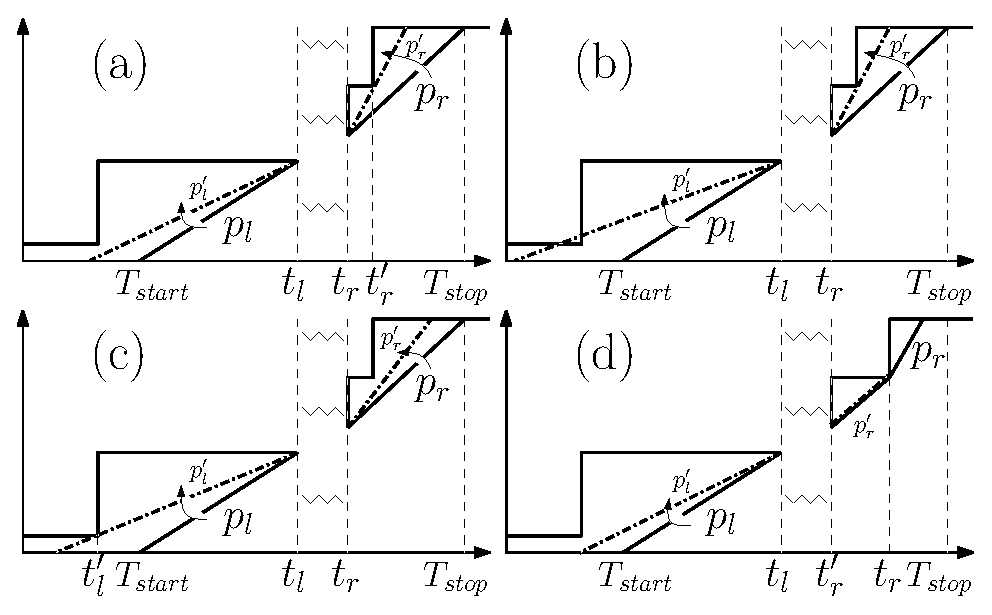
\includegraphics[width=8cm]{Algorithm1.eps}}
\caption{Figures showing any iteration of the Algorithm \ref{Algorithm1}. The solid line represents the transmission policy in the previous iteration. The dash dotted lines in (a), (b), (c), (d) represent the possible configurations of policy in the current iteration.}
\end{figure}

This is how the algorithm proceeds to generate a new transmission policy in every iteration, which begins and ends earlier than the policy given by the previous iteration, until a point is reached where either $T_{stop}-T_{start}>\TRx_0$ or $T_{start}=0$. Suppose the Algorithm terminates with $T_{start}=0$ and $T_{start}-T_{stop}\le\TRx_0$, then the policy at this iteration is the optimal policy. 


For the case where the algorithm terminates with $T_{stop}-T_{start}>\TRx_0$, let $T_{start}'$, $T_{stop}'$, $p_l'$, $p_r'$, $t_l'$, $t_r'$ be the values in the termination iteration and $T_{start}$, $T_{stop}$, $p_l$, $p_r$, $t_l$, $t_r$ be the values in the previous iteration. Then, the possible valid configurations can be one of the three shown in Fig. \ref{figure_Algorithm1} (a) (c) (d). Note that $\ETx(T_{stop}^-)=\ETx(T_{stop}'^-)$ in all the cases. (In case Fig. \ref{figure_Algorithm1} (d) we can assume that $T_{stop}'=t_r'^+$ and transmission exists after $t_r$, but with infinite power. Since transmitting with infinite power for $0$ time does not transmit any bits, we would transmit the same number of bits, as we did prior to this modification). Thus, by Lemma \ref{lemma_increase_time}, we can verify that $(T_{stop}'-T_{start}')>(T_{stop}-T_{start})$. Since $(T_{stop}'-T_{start}')\ge\TRx_0>(T_{stop}-T_{start})$, there must exist a solution to equation presented in line number \ref{algo_solve_eqn} of Algorithm \ref{Algorithm1}. Let the policy obtained from the solution start and end at $T_{start}''$ and $T_{stop}''$. Then $T_{stop}''-T_{start}''=\TRx_0$.

So we can conclude by stating that, the solution to Algorithm \ref{Algorithm1} satisfies Lemma \ref{lemma4}. Now, according to the definition of $t_n$ and $t_q$ in line number \ref{init_policy_Etn} and \ref{init_policy_t_q} of INIT\_POLICY, $t_q<t_n$. Since $t_n$ is defined as the first energy arrival epoch by which $B_0$ bits can be transmitted in $\TRx_0$ time, any transmission policy which ends at of before $t_n$ should take more than $\TRx_0$ time to transmit all of $B_0$ bits. As $t_q<t_n$, we are guaranteed that no transmission policy can finish at or before $t_q$. Hence in the iterations of the algorithm $t_r$ can never decreases beyond $t_q$. Therefore, $t_q$ always exists in the final solution to Algorithm \ref{Algorithm1}.   
